% ============================================================
% LYCANS AERODESIGN TEAM — FULL TECHNICAL REPORT
% ============================================================

% !TeX program = lualatex

\documentclass[11pt,a4paper]{article}

% ------------------------------------------------------------
% BASIC PACKAGES
% ------------------------------------------------------------

\usepackage{fontspec}
\setmainfont{Arial}

\usepackage[a4paper,margin=1in]{geometry}

\usepackage{graphicx}
\usepackage{amsmath}
\usepackage{amssymb}
\usepackage{booktabs}
\usepackage{array}
\usepackage{float}
\usepackage{enumitem}
\usepackage{xcolor}
\usepackage{hyperref}
\usepackage{listings}
\usepackage{siunitx}
\usepackage{caption}
\usepackage{fancyhdr}
\usepackage{lastpage}

% ------------------------------------------------------------
% COLORS
% ------------------------------------------------------------

\definecolor{LycansBlue}{HTML}{002060}
\definecolor{LycansLightBlue}{HTML}{203764}
\definecolor{LycansRed}{HTML}{A20000}
\definecolor{LinkBlue}{HTML}{0563C1}

% ------------------------------------------------------------
% HYPERLINKS
% ------------------------------------------------------------

\hypersetup{
    colorlinks=true,
    linkcolor=LycansBlue,
    urlcolor=LinkBlue,
    citecolor=LycansBlue
}

% ------------------------------------------------------------
% PAGE STYLE
% ------------------------------------------------------------

\pagestyle{fancy}
\fancyhf{}

% Header
\fancyhead[L]{
    \raisebox{-0.15cm}{%
        
\includegraphics[height=0.8cm]{images/lycans-logo.png}%
    }
}

\fancyhead[R]{
    \textcolor{LycansBlue}{\textbf{Full Technical Report}}
}

% Footer
\fancyfoot[C]{
    Page \thepage\ of \pageref{LastPage}
}

\renewcommand{\headrulewidth}{0.4pt}

% ------------------------------------------------------------
% SECTION STYLE
% ------------------------------------------------------------

\usepackage{titlesec}

\titleformat{\section}
    {\Large\bfseries\color{LycansBlue}}
    {\thesection}
    {0.6em}
    {}

\titleformat{\subsection}
    {\large\bfseries\color{LycansLightBlue}}
    {\thesubsection}
    {0.5em}
    {}

\titleformat{\subsubsection}
    {\normalsize\bfseries\color{LycansBlue}}
    {\thesubsubsection}
    {0.5em}
    {}

% ------------------------------------------------------------
% CODE STYLE
% ------------------------------------------------------------

\lstset{
    basicstyle=\ttfamily\small,
    breaklines=true,
    frame=single,
    columns=fullflexible
}

% ============================================================
% DOCUMENT
% ============================================================

\begin{document}

% ------------------------------------------------------------
% TITLE
% ------------------------------------------------------------

\begin{center}

    {\Large\bfseries\color{LycansBlue}
    LYCANS AERODESIGN TEAM}

    \vspace{0.5cm}

    {\LARGE\bfseries
    Powered Autonomous Delivery Aircraft (PADA) Final Technical Report}

    \vspace{0.5cm}

    \begin{tabular}{rl}
        \textbf{Group Number:} & 02 \\
    \end{tabular}

\end{center}

\vspace{0.5cm}

\hrule

\vspace{0.5cm}

% ============================================================
% SECTION 1: CONCEPTUAL DESIGN
% ============================================================

\section{Conceptual Design}
\subsection{Mission Requirements and Design Constraints}
The mission objective is to design a small unmanned aerial vehicle (UAV) resembling the Powered Autonomous Delivery Aircraft (PADA). The project simulates both aircraft design and manufacturing processes. Designing the aircraft involves integrated development of the wing, tail, fuselage, and electrical/avionics systems.

The mission operates under strict design constraints:

\begin{table}[H]
    \centering
    \caption{PADA UAV Mission and Design Constraints}
    \label{tab:mission_constraints}
    \begin{tabular}{ll}
        \toprule
        \textbf{Parameter} & \textbf{Constraint} \\
        \midrule
        Maximum Wingspan & 25 in \\ 
        Maximum Gross Weight & 19.5 oz ($\approx$553 g, including electrical system) \\ 
        Payload & Empty Pepsi can (external release mechanism) \\ 
        Wing Airfoil Options & E423, S1223, GOE 165, or NACA 2412 \\ 
        Battery Energy Limit & $\le \SI{100}{\watt\hour}$ (LiHV prohibited) \\ 
        Takeoff Ground Distance & \SI{8}{\meter} to \SI{12}{\meter} \\ 
        Takeoff Angle of Attack & $< 35^\circ$ to $40^\circ$ \\ 
        Minimum Cruise Speed & \SI{25}{\meter\per\second} \\ 
        Minimum Turn Bank Angle & $> 60^\circ$ \\ 
        Flight Altitude Range & \SI{50}{\meter} to \SI{100}{\meter} \\ 
        \bottomrule
    \end{tabular}
\end{table}

\subsection{Selected Aircraft Configuration}
\subsubsection{Airfoil Selection}
The chosen airfoil for the PADA's wing is the **S1223 Airfoil**, selected based on a trade study comparing lift efficiency and low-Reynolds-number behavior:

\begin{figure}[H]
    \centering
    \begin{minipage}{0.45\textwidth}
        \centering
        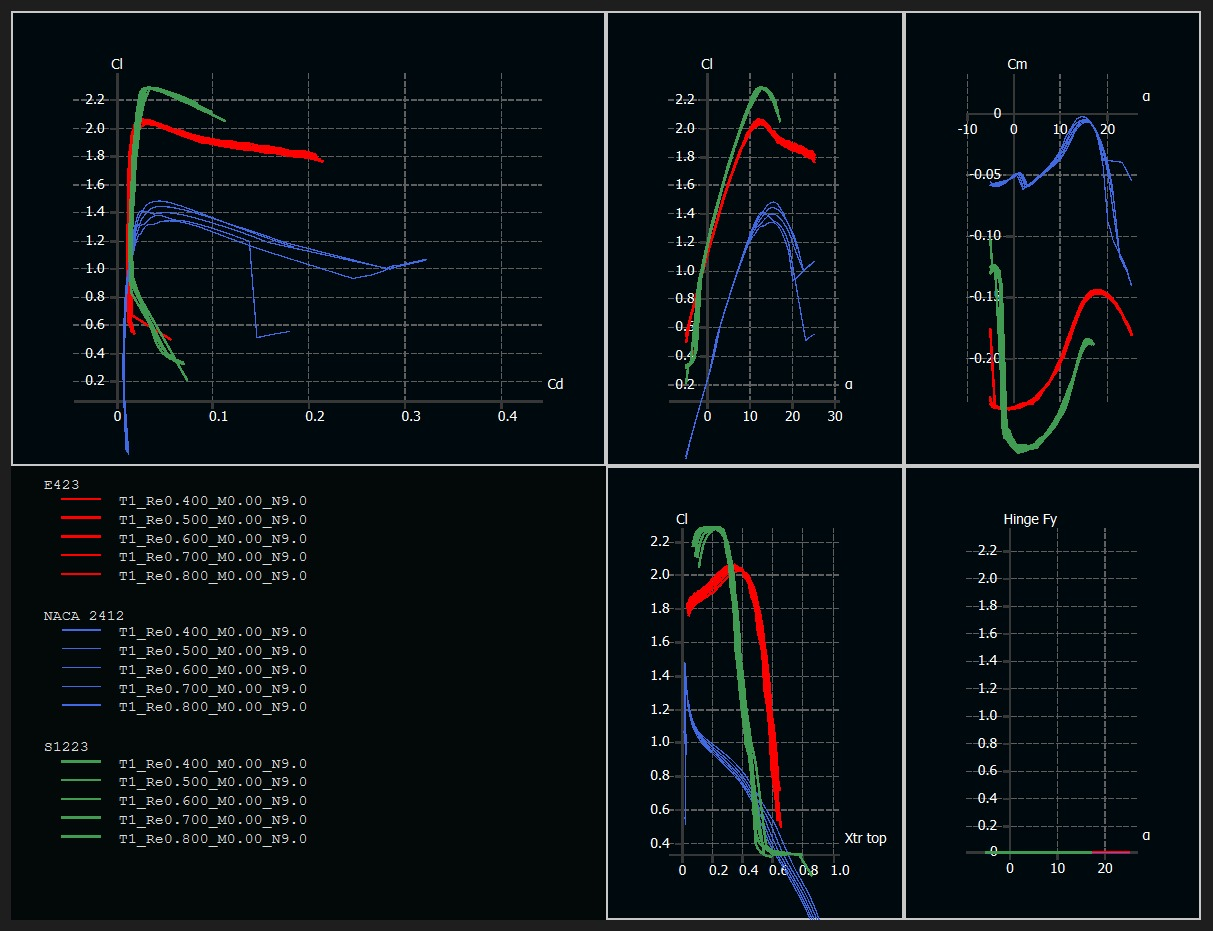
\includegraphics[width=\textwidth]{images/Airfoil Analysis.jpg}
        \caption{Airfoil Analysis and Comparison}
    \end{minipage}
    \hfill
    \begin{minipage}{0.45\textwidth}
        \centering
        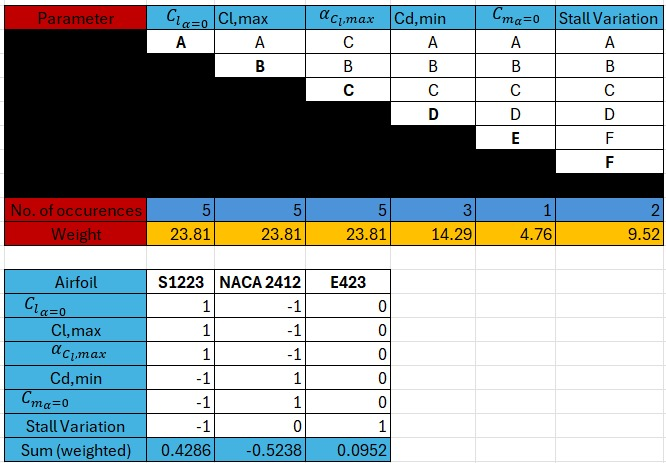
\includegraphics[width=\textwidth]{images/Airfoil Tradestudy.jpg}
        \caption{Airfoil trade study}
    \end{minipage}
\end{figure}

\subsubsection{Wing and Tail Configurations}
A conventional low-wing monoplane configuration with a single tractor propeller was selected for maximum structural efficiency and clean airflow over the tail control surfaces.

\subsubsection{Fuselage}
The fuselage is designed as an enclosed rectangular box structure to optimize internal volume for battery placement along the Center of Gravity (CG) tray and to allow direct belly-mounting of the payload release mechanism.

% ============================================================
% SECTION 2: PRELIMINARY DESIGN
% ============================================================

\section{Preliminary Design}
\subsection{Propulsion Constraint Analysis}
Constraint analysis was conducted based on Takeoff, Cruise, Landing, and Turning regimes:

\begin{figure}[H]
    \centering
    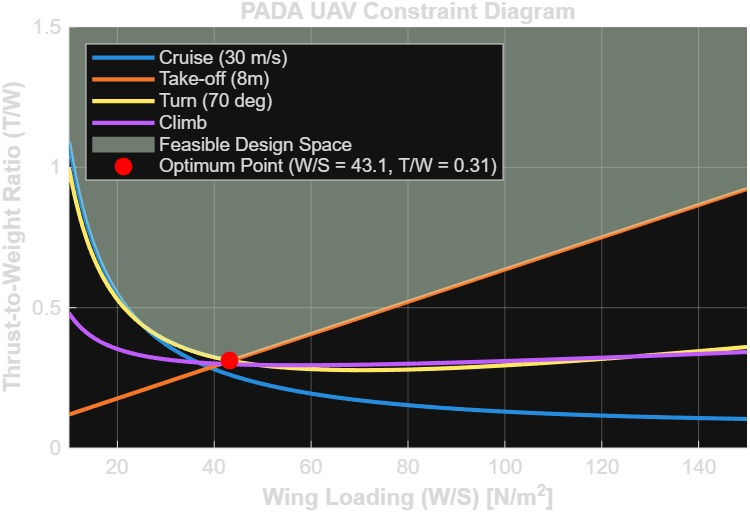
\includegraphics[width=0.6\textwidth]{images/Constraint Analysis.jpg}
    \caption{Propulsion constraint analysis diagram showing the design point.}
    \label{fig:constraint_analysis}
\end{figure}

The optimum operating point is highlighted where Wing Loading is $43.1$ and Thrust-to-Weight ratio is $0.31$. This analysis assumes an Aspect Ratio ($AR$) of $3.33$, a climb rate of $\SI{3}{\meter\per\second}$, and a turn radius $R = \SI{30}{\meter}$.

\subsection{Wing and Tail Sizing}
Wing geometry was constrained to a maximum wingspan of $25\,\text{in}$ ($\SI{0.635}{\meter}$). The wing area $S$ was derived from the target wing loading to ensure adequate lift at cruise speeds above $\SI{25}{\meter\per\second}$.

\subsection{Aerodynamic Modeling and Stability Analysis (XFLR5)}
To evaluate aerodynamic performance and both static and dynamic stability, the aircraft was modeled in XFLR5.

\subsubsection{Design Iterations and Configuration Selection}
\begin{itemize}
    \item \textbf{Dihedral Angle:} Dihedral was initially considered but eliminated to simplify laser-cut manufacturing. The final aircraft uses a flat wing.
    \item \textbf{Tail Arm Length:} A moderate tail arm length was maintained to keep the horizontal tail volume coefficient ($V_h$) balanced without causing excessive stability that would degrade pitch responsiveness.
    \item \textbf{Center of Gravity and Static Margin:} Component placement yields a final static margin of exactly 24\%.
\end{itemize}

\subsubsection{Analysis and Eigenmode Evaluation}
Dynamic stability analysis confirmed positive damping across both lateral and longitudinal modes:

\begin{figure}[H]
    \centering
    \begin{minipage}{0.48\textwidth}
        \centering
        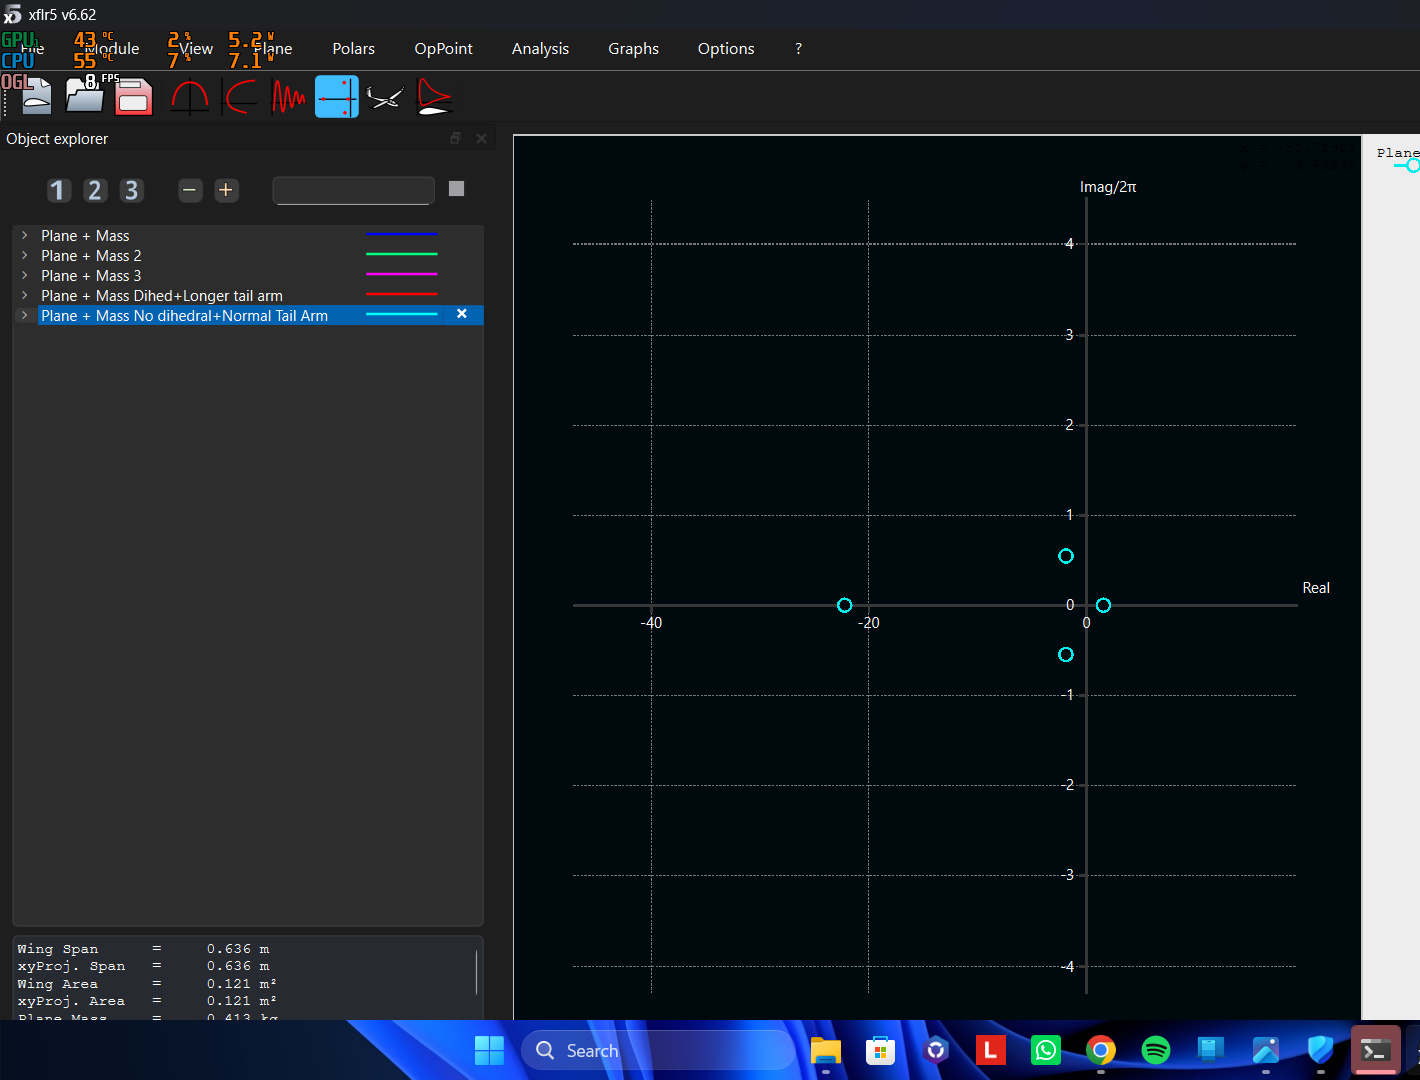
\includegraphics[width=\textwidth]{images/Lateral.png}
        \caption{Lateral dynamic stability eigenmodes.}
    \end{minipage}
    \hfill
    \begin{minipage}{0.48\textwidth}
        \centering
        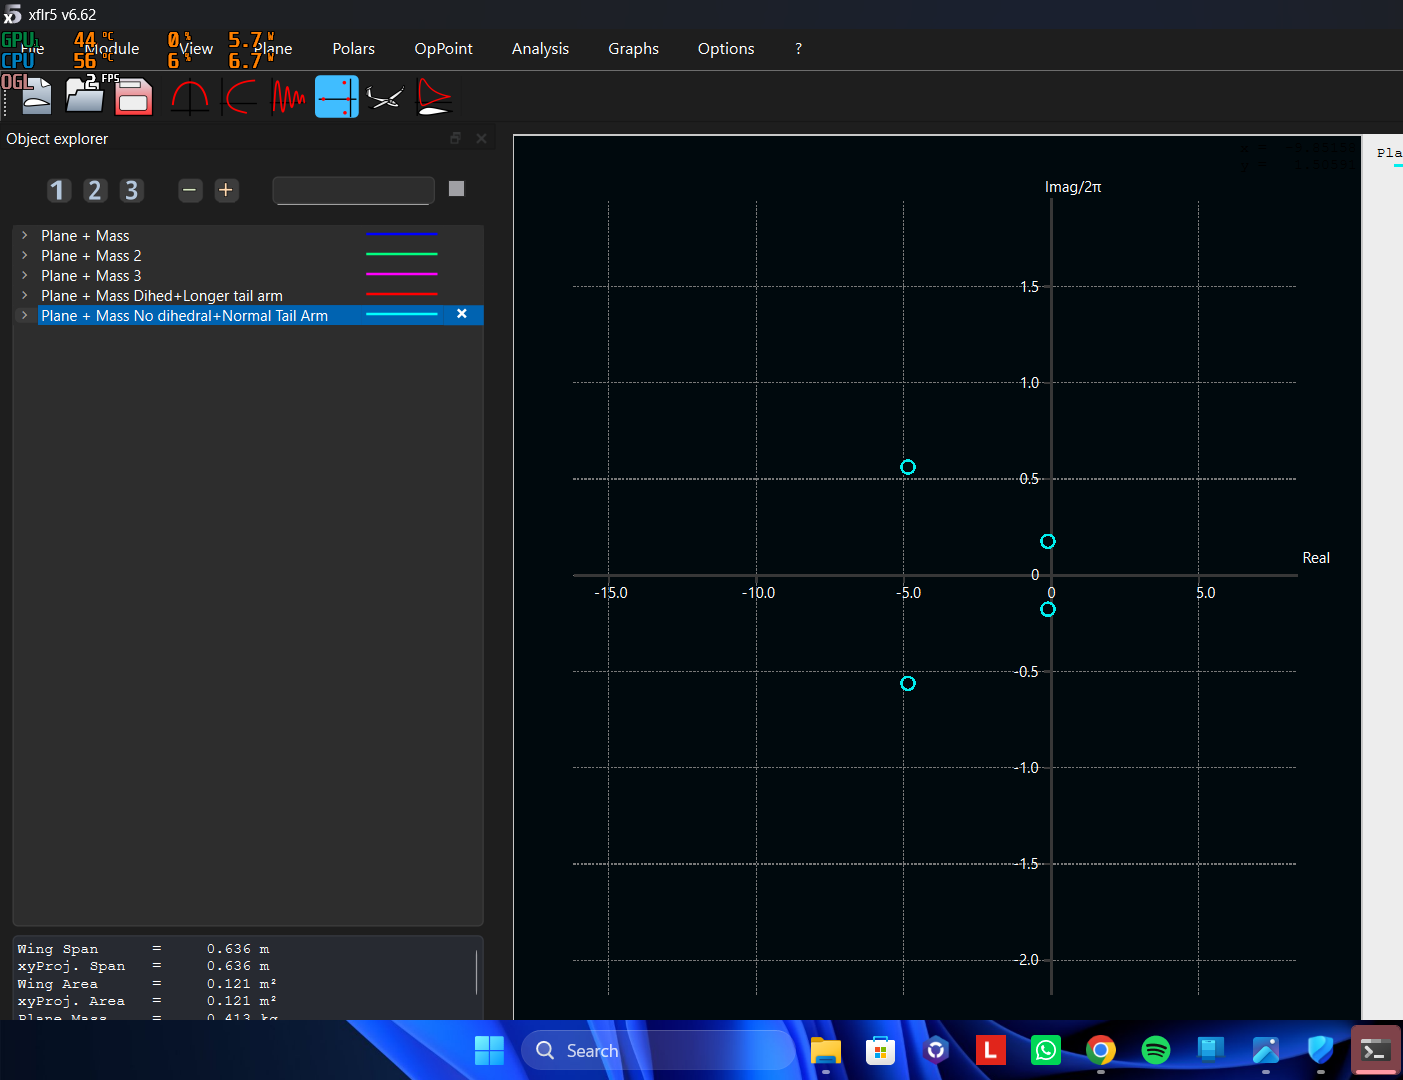
\includegraphics[width=\textwidth]{images/Longitudinal.png}
        \caption{Longitudinal dynamic stability eigenmodes.}
    \end{minipage}
\end{figure}

\begin{figure}[H]
    \centering
    \includegraphics[width=0.75\textwidth]{images/polars.png}
    \caption{Aerodynamic performance polars across varying angles of attack.}
    \label{fig:polars}
\end{figure}

\subsection{Aircraft Design}
\begin{figure}[H]
    \centering
    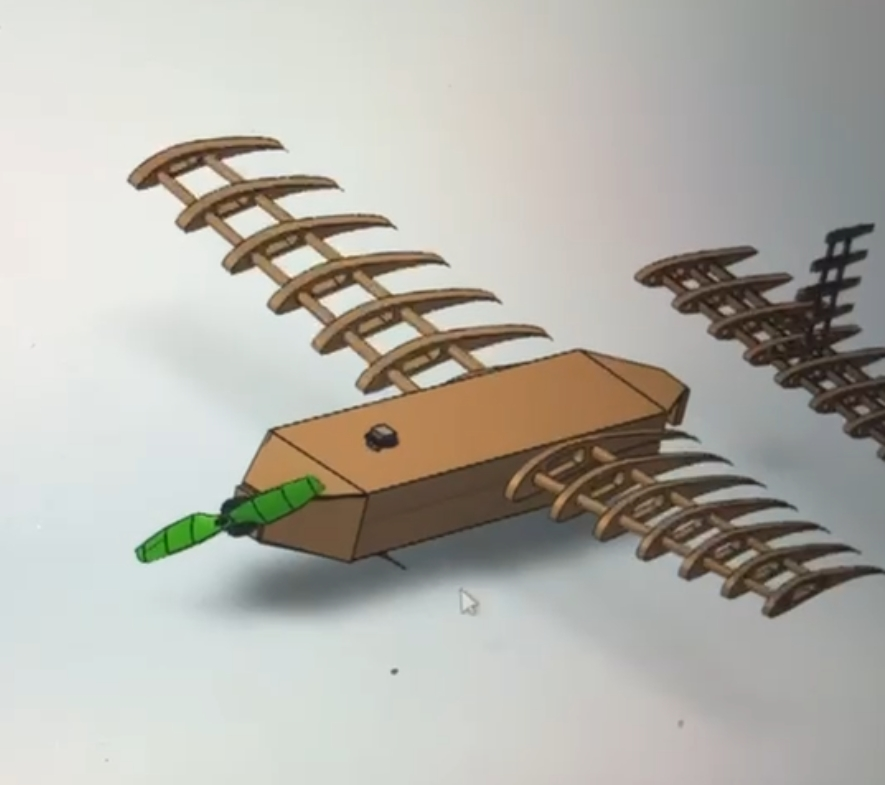
\includegraphics[width=0.75\textwidth]{images/Solid.jpg}
    \caption{SolidWorks CAD integration of the airframe.}
    \label{fig:solidworks}
\end{figure}

\begin{figure}[H]
    \centering
    \begin{minipage}{0.48\textwidth}
        \centering
        \includegraphics[width=\textwidth]{images/wing.png}
        \caption{Final main wing configuration.}
    \end{minipage}
    \hfill
    \begin{minipage}{0.48\textwidth}
        \centering
        \includegraphics[width=\textwidth]{images/cg.png}
        \caption{Final Center of Gravity placement (24\% static margin).}
    \end{minipage}
\end{figure}

\begin{figure}[H]
    \centering
    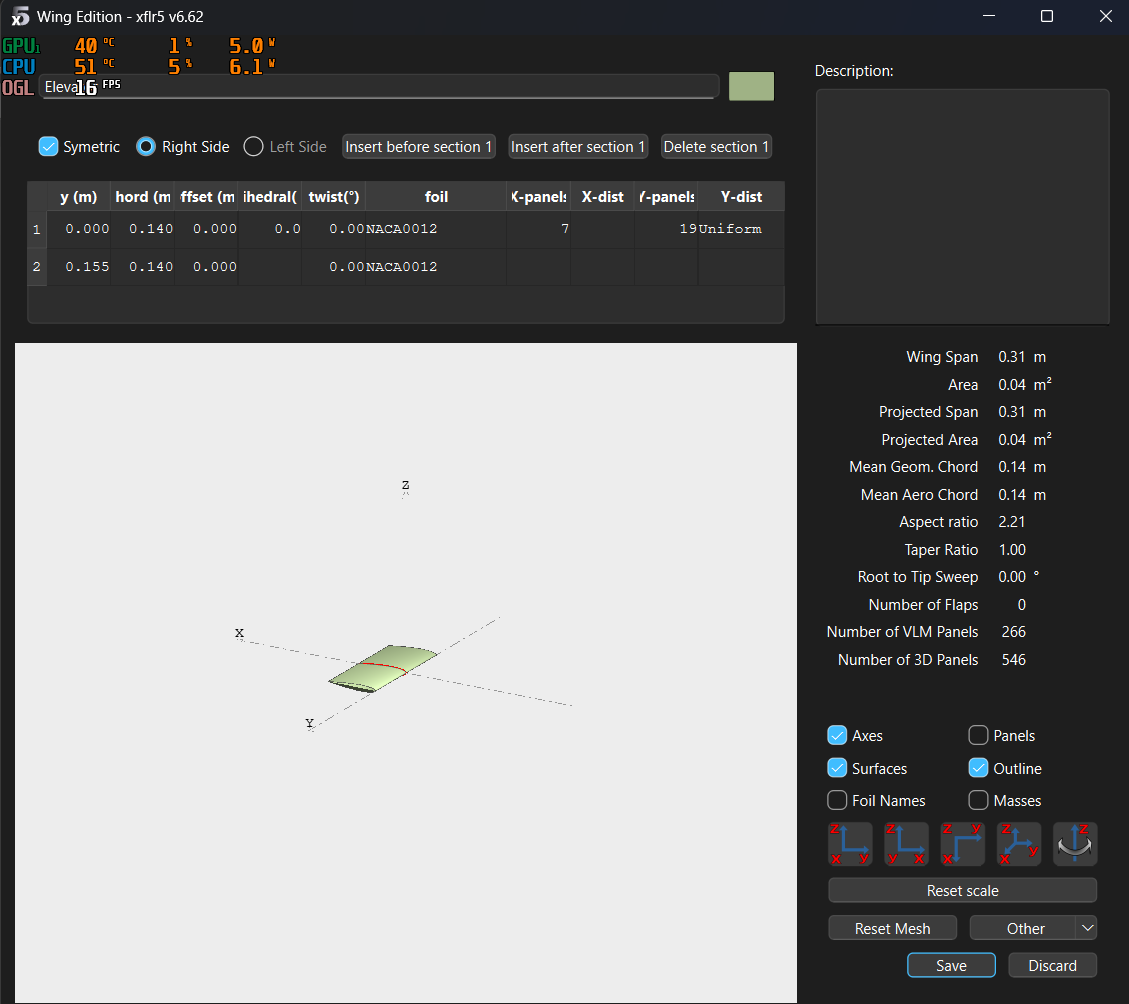
\includegraphics[width=0.4\textwidth]{images/H Tail.png}
    \hspace{0.5cm}
    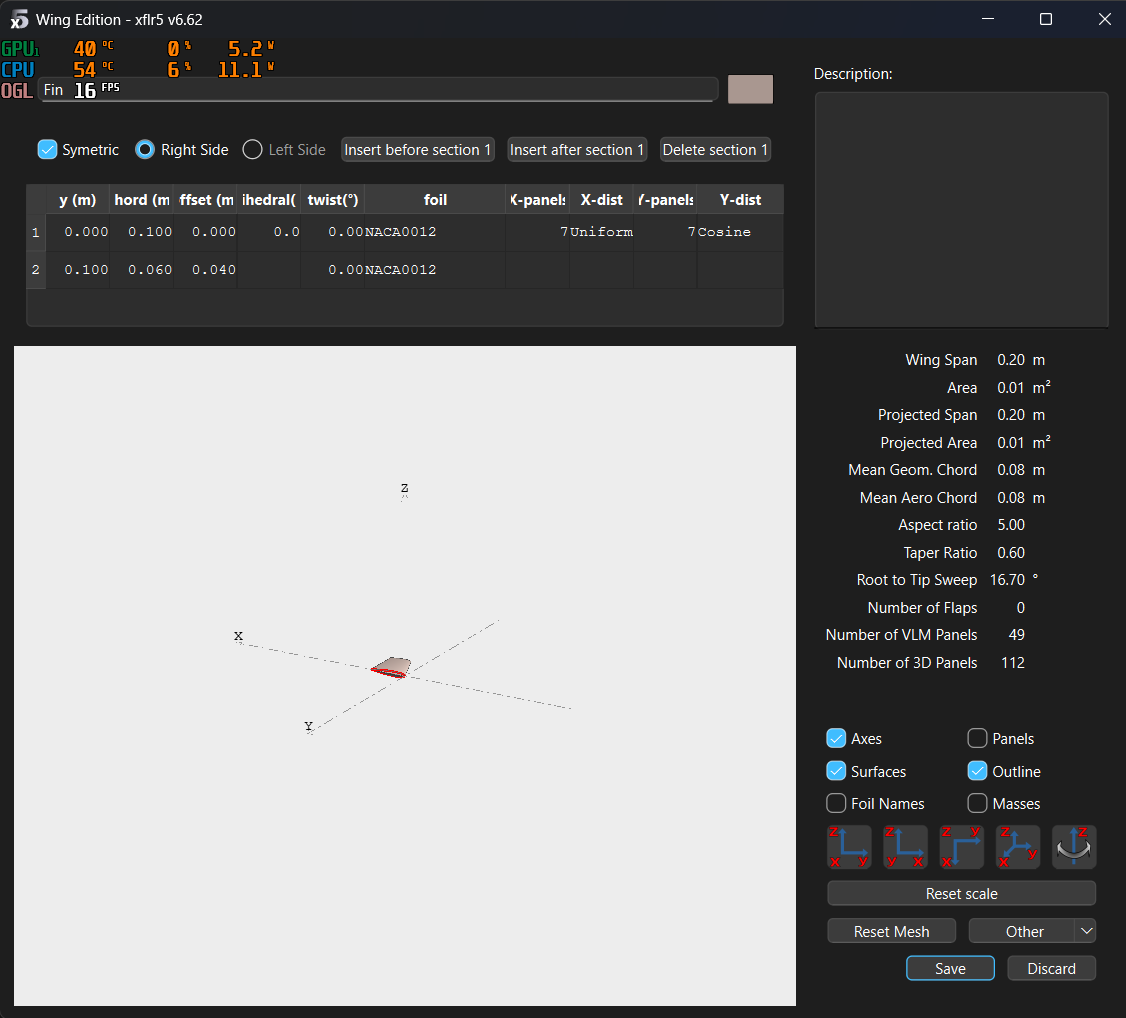
\includegraphics[width=0.4\textwidth]{images/V Tail.png}
    \caption{Final horizontal and vertical empennage design.}
    \label{fig:final_tail}
\end{figure}

% ============================================================
% SECTION 3: DETAIL MECHANICAL & STRUCTURAL DESIGN
% ============================================================

\section{Detail Mechanical \& Structural Design}

\subsection{Payload Release Mechanism}
\subsubsection{Final CAD Design and Release Principle}

\begin{figure}[H]
    \centering
    
\includegraphics[width=0.55\textwidth]{images/Payload Mech.png}
    \caption{Payload release mechanism assembly components.}
    \label{fig:payload_mech}
\end{figure}

The external payload mechanism comprises three primary structural parts:
\begin{itemize}
    \item Movable Arm (actuated via a micro servo)
    \item Fixed Arm
    \item Back Support
\end{itemize}

\textbf{Operation:} A dedicated fifth micro servo rotates the movable arm outward to drop the payload. The static back support maintains payload alignment during flight maneuvers. The assembly is mounted directly under the aircraft CG to ensure the 24\% static margin remains unchanged before and after release.

\subsection{Material Selection}
Balsa wood was selected for all airframe components due to its high strength-to-weight ratio, low cost, and ease of laser cutting. This keeps total structural weight minimal while safely withstanding flight loads.

% ============================================================
% SECTION 4: HARDWARE REQUIREMENTS
% ============================================================

\section{Hardware Requirements}

\subsection{Electrical and Avionics Design}
The electrical architecture delivers regulated power to high-draw propulsion components and sensitive digital avionics while maintaining strict weight and safety margins.

\subsubsection{Component Selection and Power Budget}
A detailed power and weight budget was established to size the battery and verify system stability under peak loads:

\begin{table}[H]
    \centering
    \caption{PADA Electrical Components Inventory}
    \label{tab:power_budget}
    \small
    \begin{tabular}{l l l l l}
        \toprule
        \textbf{Component} & \textbf{Power or Amp Rating} & \textbf{Price} & \textbf{Weight} & \textbf{Selected Model / Notes} \\
        \midrule
        Battery & 11.1V 3S 850mAh 75C & \$14.00 & 85 g & Tattu High-C Micro LiPo \\
        ESC & 30A Cont. (40A Burst) & \$12.00 & 18 g & BLHeli\_S 30A Slim ESC \\
        Motor & 2205 2300KV (Max 22A) & \$14.00 & 30 g & EMAX RS2205 Outrunner \\
        Propeller & N/A & \$3.00 & 6 g & Gemfan 6040 2-Blade Light \\
        Flight Controller & 5.0V DC / 2W & \$48.00 & 10 g & Matek H743-WING (ArduPilot) \\
        Receiver & 5.0V DC / 100mW & \$12.00 & 7 g & ExpressLRS EP1 Receiver \\
        Telemetry & 5.0V DC / 100mW & (included) & (shared) & ExpressLRS EP1 (combined RC + telemetry link) \\
        GPS Module & 5.0V DC / 100mA & \$20.00 & 11 g & Matek M10Q-5883 Micro \\
        Servos (x4) & 4.8V--6.0V DC ($1.8\,\text{kg}\cdot\text{cm}$) & \$16.00 & 36 g & 4x 9g Metal Gear Micro \\
        \midrule
        \textbf{Total System} & --- & \textbf{\$139.00} & \textbf{203 g} & \textbf{Compliant} \\
        \bottomrule
    \end{tabular}
\end{table}

\noindent
\textit{Note: ExpressLRS EP1 provides both RC control and telemetry over a single radio link; it is listed twice above to match category accounting while sharing mass and cost.}

\noindent
\textit{Note: The 203\,g electrical mass leaves ample margin for the structural frame within the 19.5\,oz ($\approx$553\,g) maximum gross weight budget.}

\textbf{Battery Endurance Calculation:}
At a continuous nominal cruise draw of $9.28\,\text{A}$ on an $850\,\text{mAh}$ battery, nominal operational flight time $t_{\text{flight}}$ is:
\begin{equation}
    t_{\text{flight}} = \frac{0.85\,\text{Ah} \times 0.80 \text{ (usable capacity)}}{9.28\,\text{A}} \times 60\,\text{min/hr} \approx 4.40\,\text{minutes}
\end{equation}
This satisfies the 3--5 minute mission window with a 20\% capacity buffer. Total battery energy ($11.1\text{V} \times 0.85\text{Ah} \approx 9.4\,\text{Wh}$) complies with the $\le 100\,\text{Wh}$ limit.

\subsubsection{Electrical Block Diagram and Schematic}

\begin{figure}[H]
    \centering
    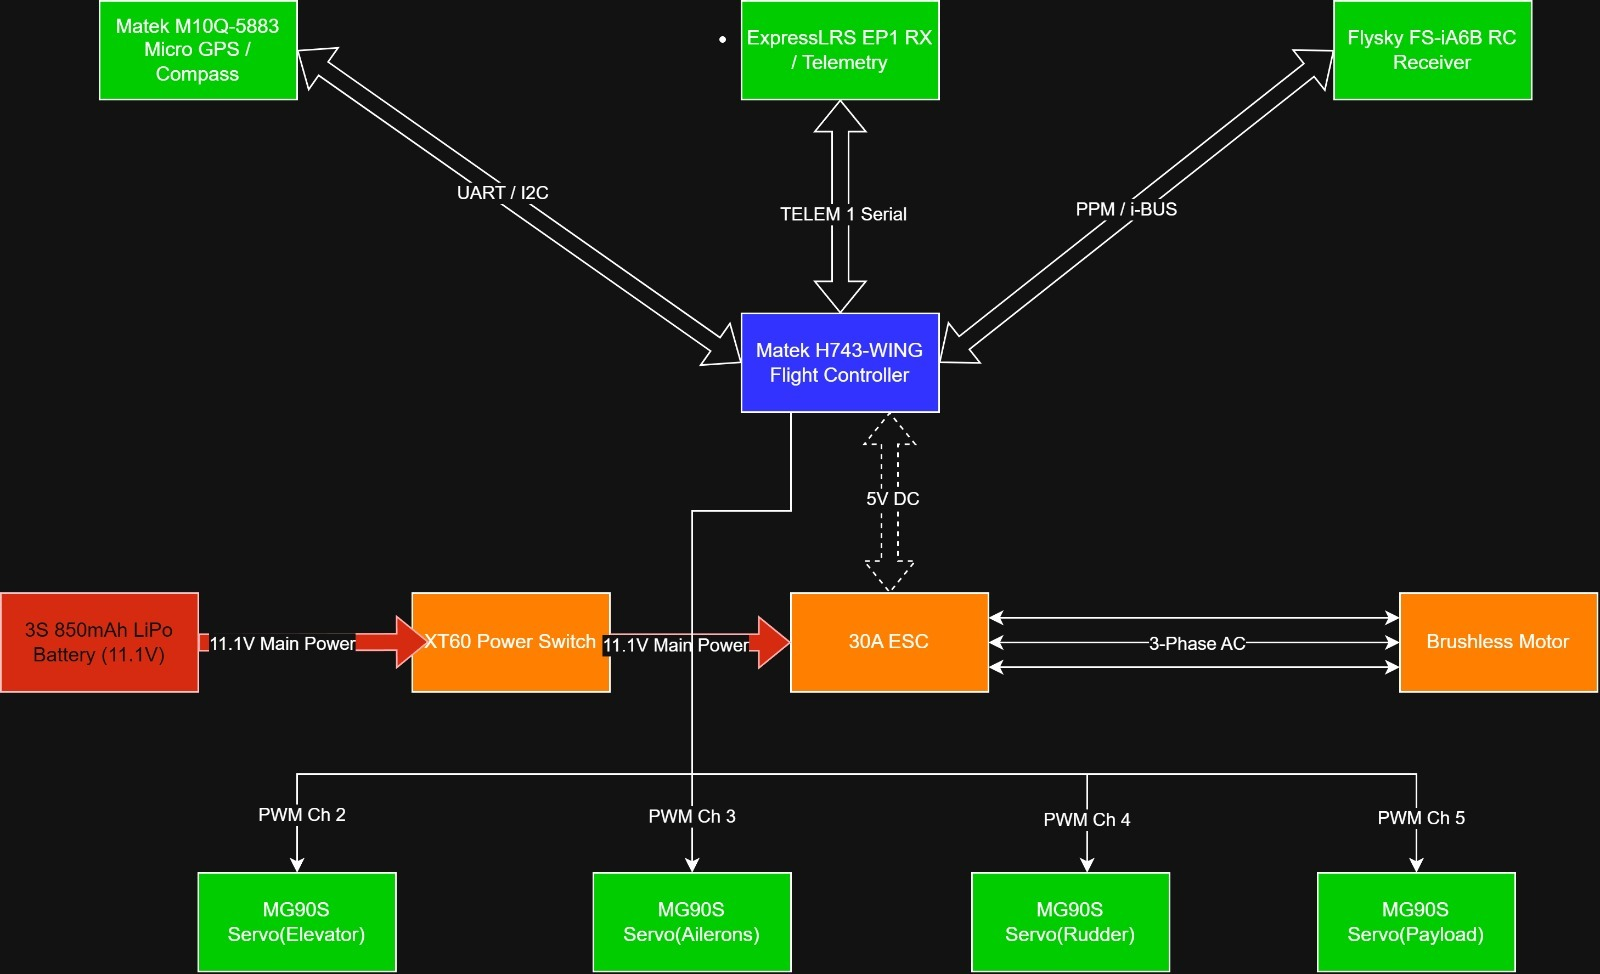
\includegraphics[width=0.85\linewidth]{images/hardware.jpeg}
    \caption{PADA Aircraft Electrical System Block Diagram and Interconnects.}
    \label{fig:elec_schematic}
\end{figure}

\subsubsection{Wiring, Connectors, Protection, and Electrical Safety}
\begin{itemize}
    \item \textbf{High-Current Path:} 16 AWG silicone wire rated for up to $30\,\text{A}$ continuous connects the LiPo to the ESC via an XT30 connector.
    \item \textbf{Low-Voltage Signal Path:} 26 AWG twisted-pair wires minimize EMI on signal lines.
    \item \textbf{Voltage Regulation:} The ESC's integrated 5V BEC powers the flight controller, receiver, and servos. An inline capacitor suppresses voltage spikes during sudden throttle bursts.
\end{itemize}

\subsubsection{Component Placement and Integration}
\begin{itemize}
    \item \textbf{CG Alignment:} The 3S LiPo ($85\,\text{g}$) and Matek FC ($10\,\text{g}$) sit on an adjustable tray directly over the calculated CG.
    \item \textbf{Vibration Isolation:} The flight controller is mounted on anti-vibration foam tape.
    \item \textbf{EMI Separation:} The Matek M10Q GPS module is elevated on a 10\,cm carbon mast clear of high-current power cables.
\end{itemize}

% ============================================================
% SECTION 5: SOFTWARE REQUIREMENTS
% ============================================================

\section{Software Requirements}

\subsection{MAVROS Installation \& SITL Connection}
MAVROS was installed via ROS 2 Jazzy repositories and linked to ArduPilot SITL (ArduPlane) over UDP. Proper connectivity was verified by monitoring \texttt{/mavros/state} for a \texttt{connected: true} response.

\subsection{Autonomous Mission Adaptation via Visual Perception}

\subsubsection{Physical System Setup \& SITL Architecture}
\begin{itemize}
    \item \textbf{Physical Optical Sensing:} A smartphone running IP Webcam streams live video over HTTP to OpenCV's \texttt{VideoCapture} interface.
    \item \textbf{Companion Workstation:} Ubuntu 24.04 running ROS 2 Jazzy executes \texttt{camera\_publisher\_node} to publish frames on \texttt{/camera/image\_raw}.
    \item \textbf{ROS 2 / MAVROS Middleware:} The \texttt{vision\_processor\_node} subscribes to images, processes visual cues, and sends mode change requests to MAVROS (\texttt{/mavros/set\_mode}).
    \item \textbf{Flight Execution \& Telemetry:} Simulated ArduPlane executes flight mode changes in SITL while telemetry is monitored in QGroundControl.
\end{itemize">

\subsubsection{Unified Mission Scenario \& Perception Requirements}
A unified vision pipeline executes two real-time behaviors during mission flight:
\begin{enumerate}
    \item \textbf{Environmental Hazard / Obstacle Avoidance:} When a red object is detected, the mode switches to \texttt{GUIDED} to halt waypoint progression. Once the hazard clears, it reverts to \texttt{AUTO}.
    \item \textbf{Visual Mission Instruction:} Detecting a blue object triggers a mode switch to \texttt{RTL} via \texttt{/mavros/set\_mode}.
\end{enumerate}

\begin{table}[H]
\centering
\begin{tabular}{|l|l|l|}
\hline
\textbf{Visual Cue} & \textbf{Interpretation} & \textbf{Resulting Flight Mode} \\
\hline
Red object detected & Environmental hazard & \texttt{GUIDED} (evasive) \\
\hline
Hazard cleared (no red) & Path clear & \texttt{AUTO} (resume mission) \\
\hline
Blue object detected & Visual Target A (mission command) & \texttt{RTL} \\
\hline
No recognizable cue & Normal monitoring & No action taken \\
\hline
\end{tabular}
\caption{Target-to-flight-mode mapping used by \texttt{vision\_processor\_node}.}
\label{tab:target_mapping}
\end{table}

\subsubsection{System Architecture \& ROS 2 Interface Design}

\begin{itemize}
    \item \textbf{\texttt{camera\_publisher\_node}:} Captures $640\times480$ frames at 30~FPS and publishes to \texttt{/camera/image\_raw}.
    
    \begin{figure}[H]
        \centering
        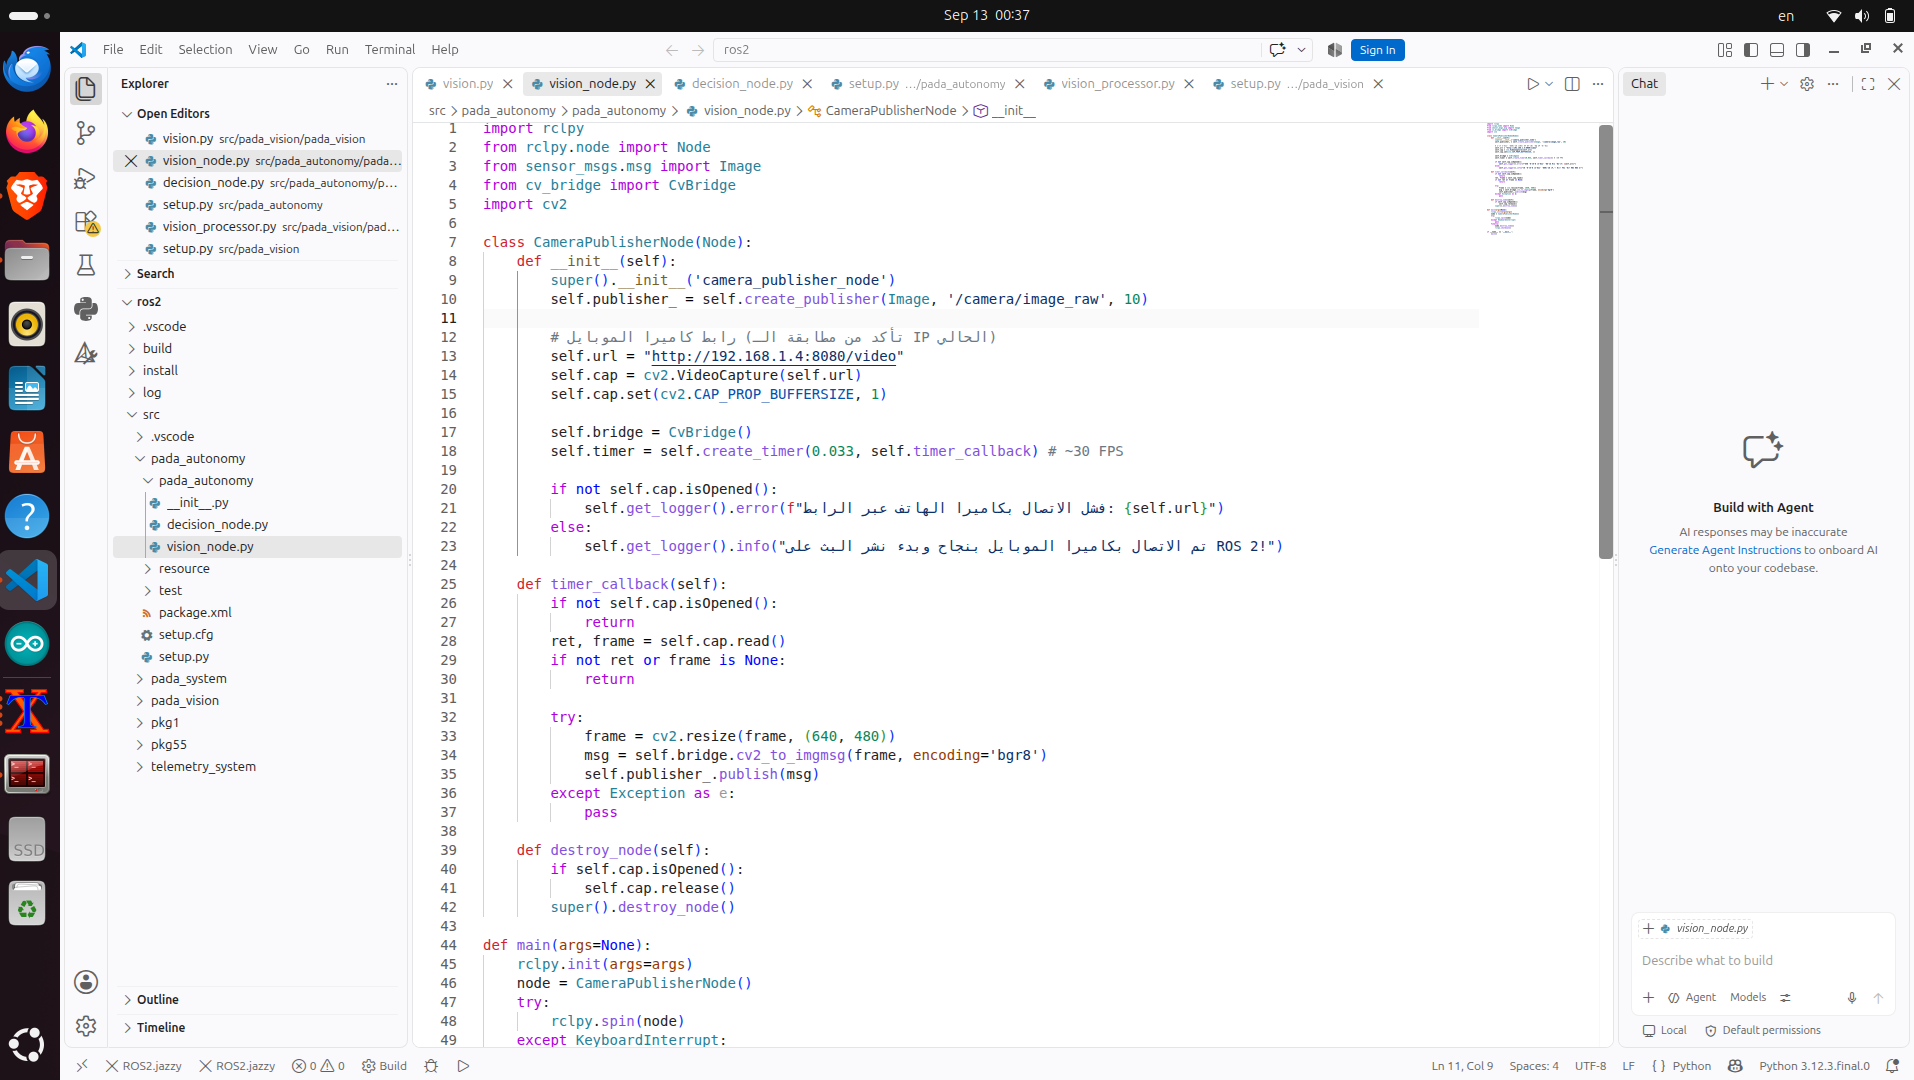
\includegraphics[width=0.7\linewidth]{images/PUBLISH.png}
        \caption{\texttt{camera\_publisher\_node} frame acquisition.}
        \label{fig:publish}
    \end{figure}

    \item \textbf{\texttt{vision\_processor\_node}:} Applies HSV thresholding and calls MAVROS services.

    \begin{figure}[H]
        \centering
        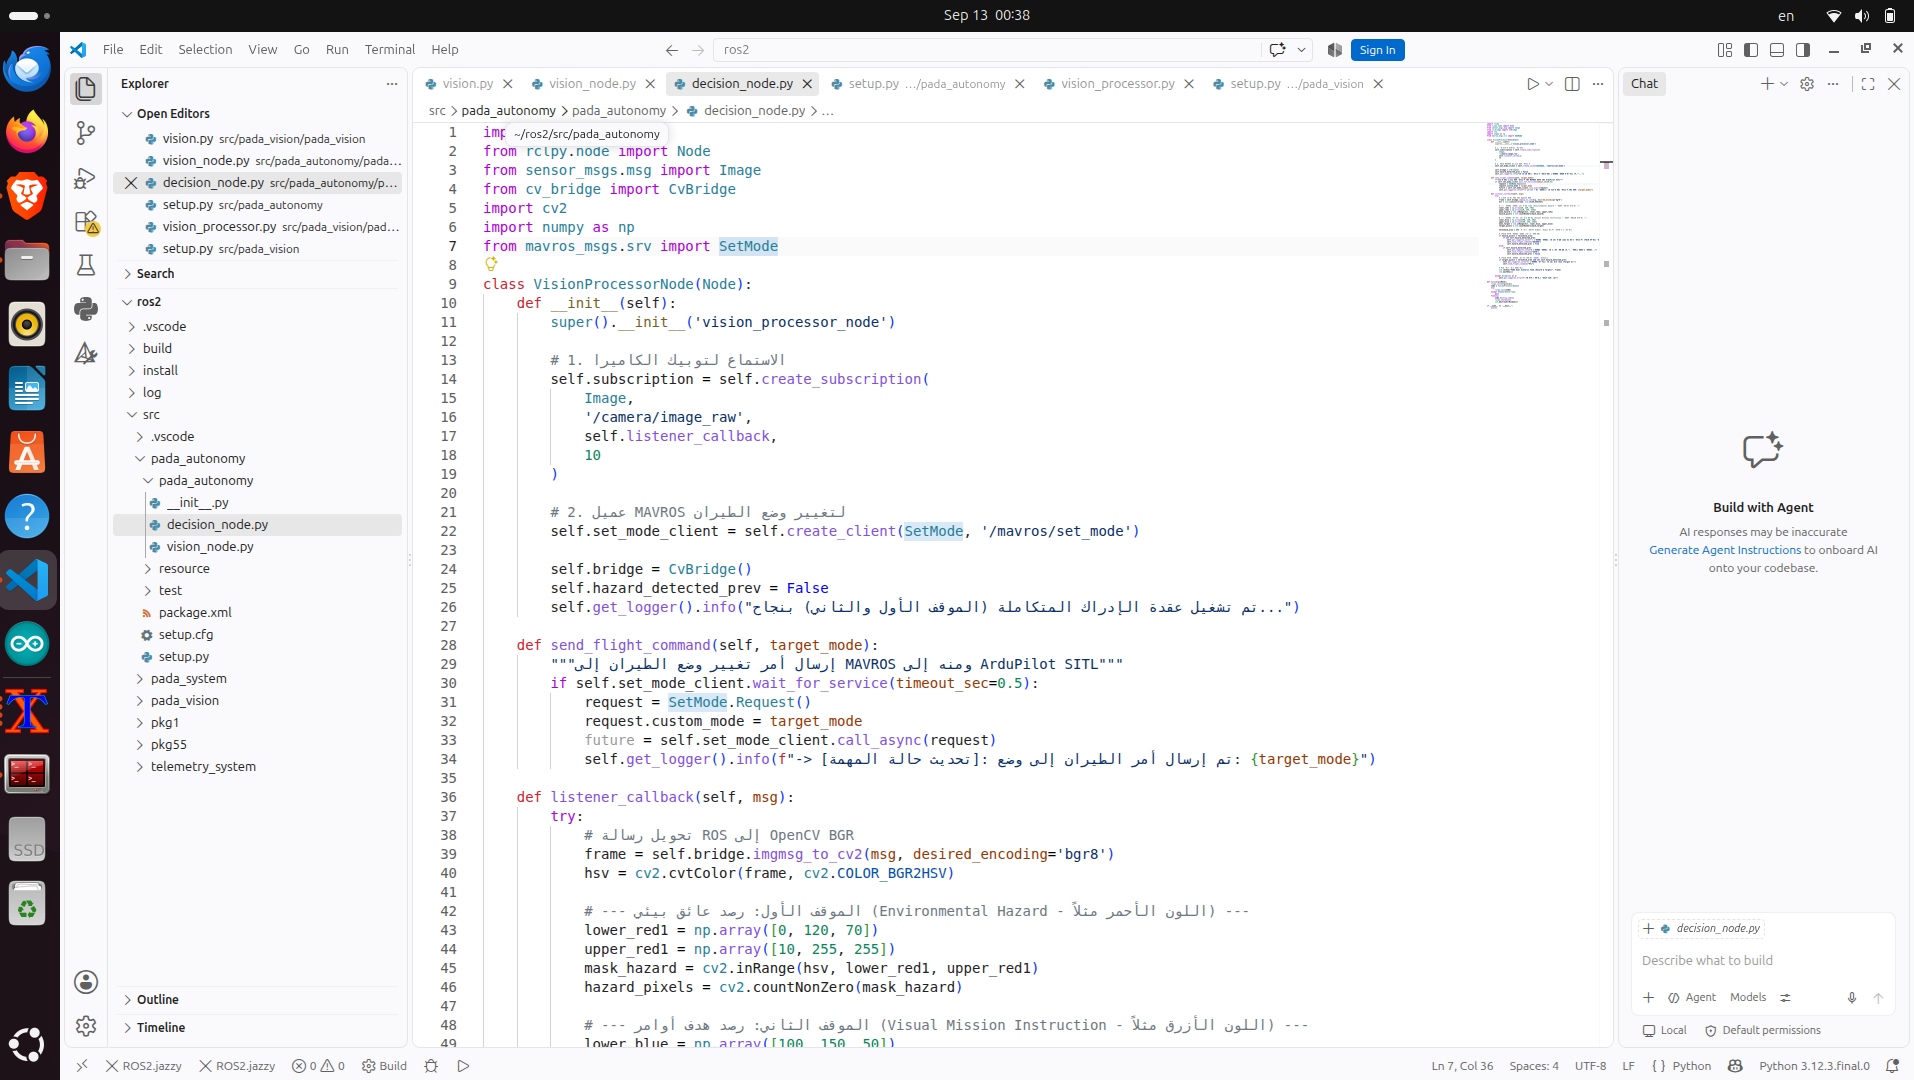
\includegraphics[width=0.7\linewidth]{images/SUBSCRIBE.png}
        \caption{\texttt{vision\_processor\_node} topic processing.}
        \label{fig:subscribe}
    \end{figure}
\end{itemize}

\begin{figure}[H]
    \centering
    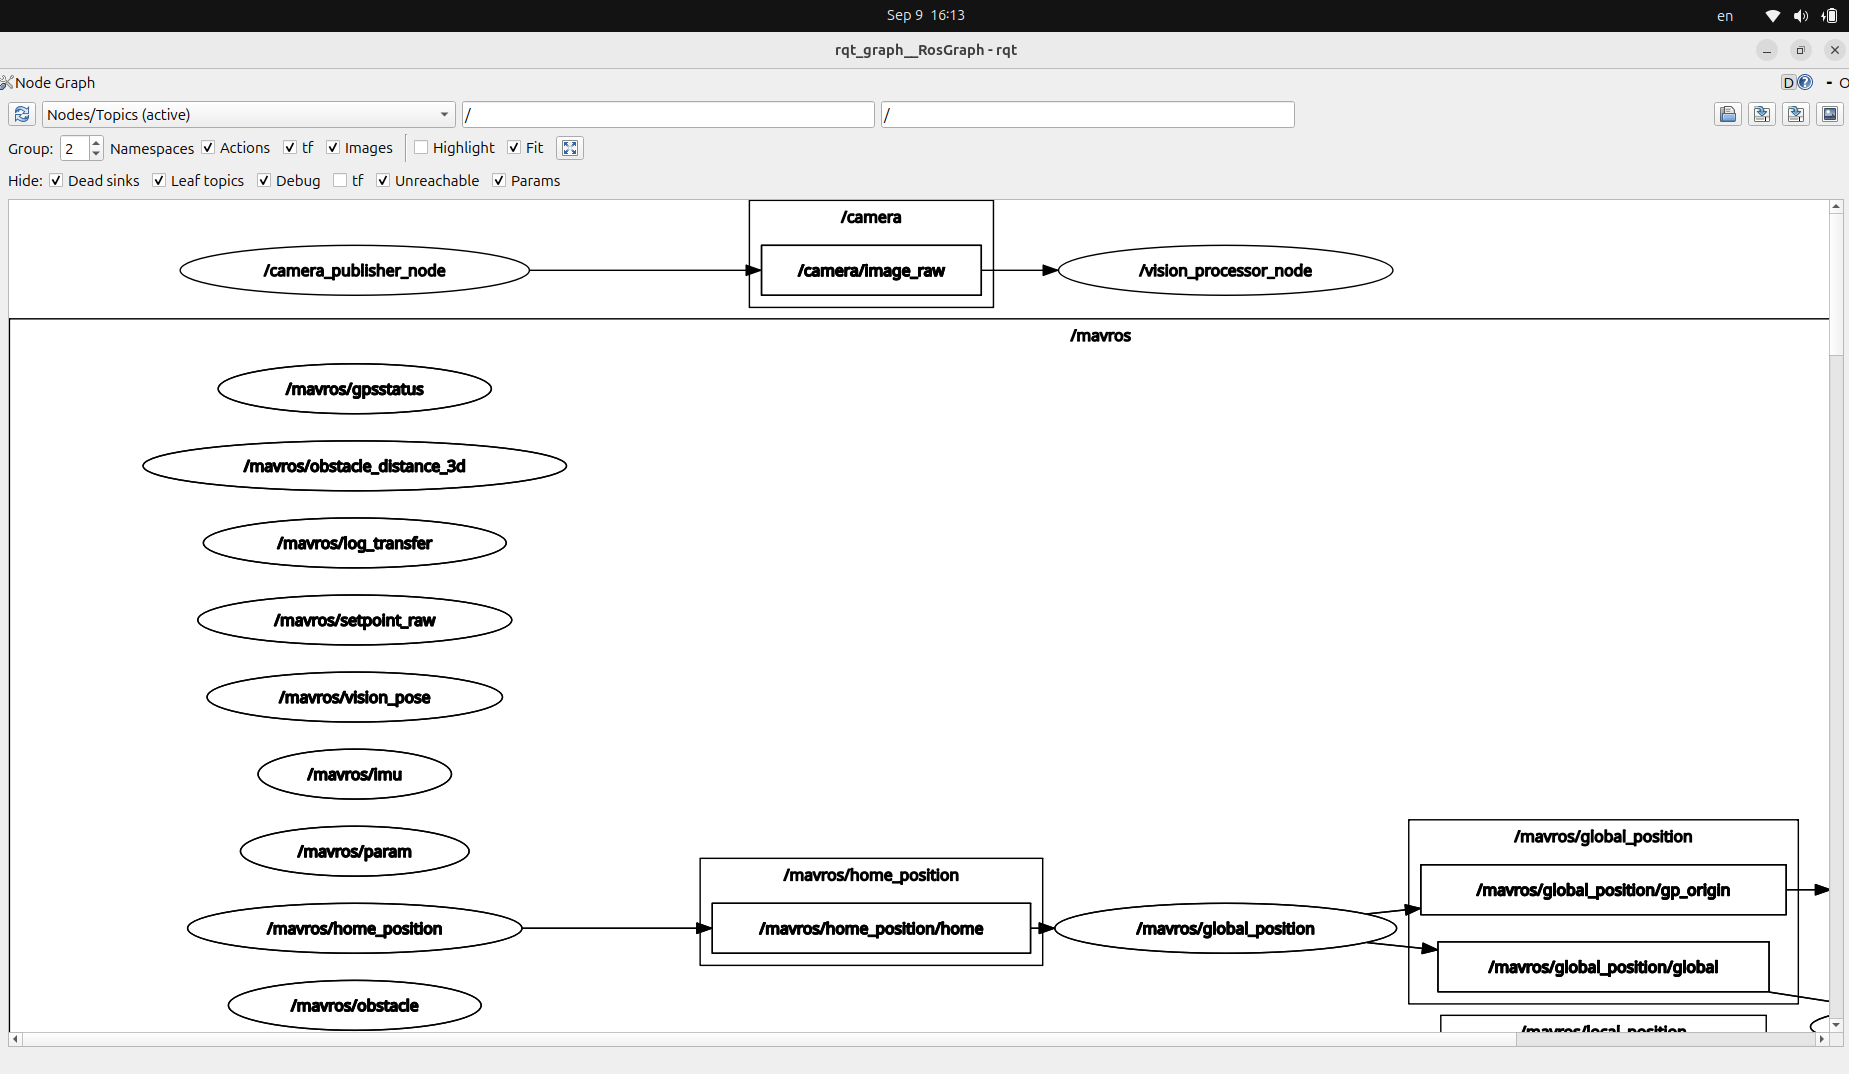
\includegraphics[width=0.7\textwidth]{images/rqt_graph.png}
    \caption{\texttt{rqt\_graph} showing node communication graph.}
    \label{fig:rqtgraph}
\end{figure}

\subsubsection{Engineering Justifications \& Tradeoff Defense}
\begin{itemize}
    \item \textbf{Perception Strategy:} HSV color space isolates Hue from lighting changes.
    \item \textbf{Filtering:} A minimum contour threshold of $600\text{ pixels}$ prevents noise triggers.
    \item \textbf{Efficiency:} Frame buffer size set to 1 (\texttt{CAP\_PROP\_BUFFERSIZE = 1}) prevents frame latency.
\end{itemize}

\subsubsection{Demonstration \& Validation Protocol}
\begin{figure}[H]
    \centering
    \begin{minipage}{0.32\textwidth}
        \centering
        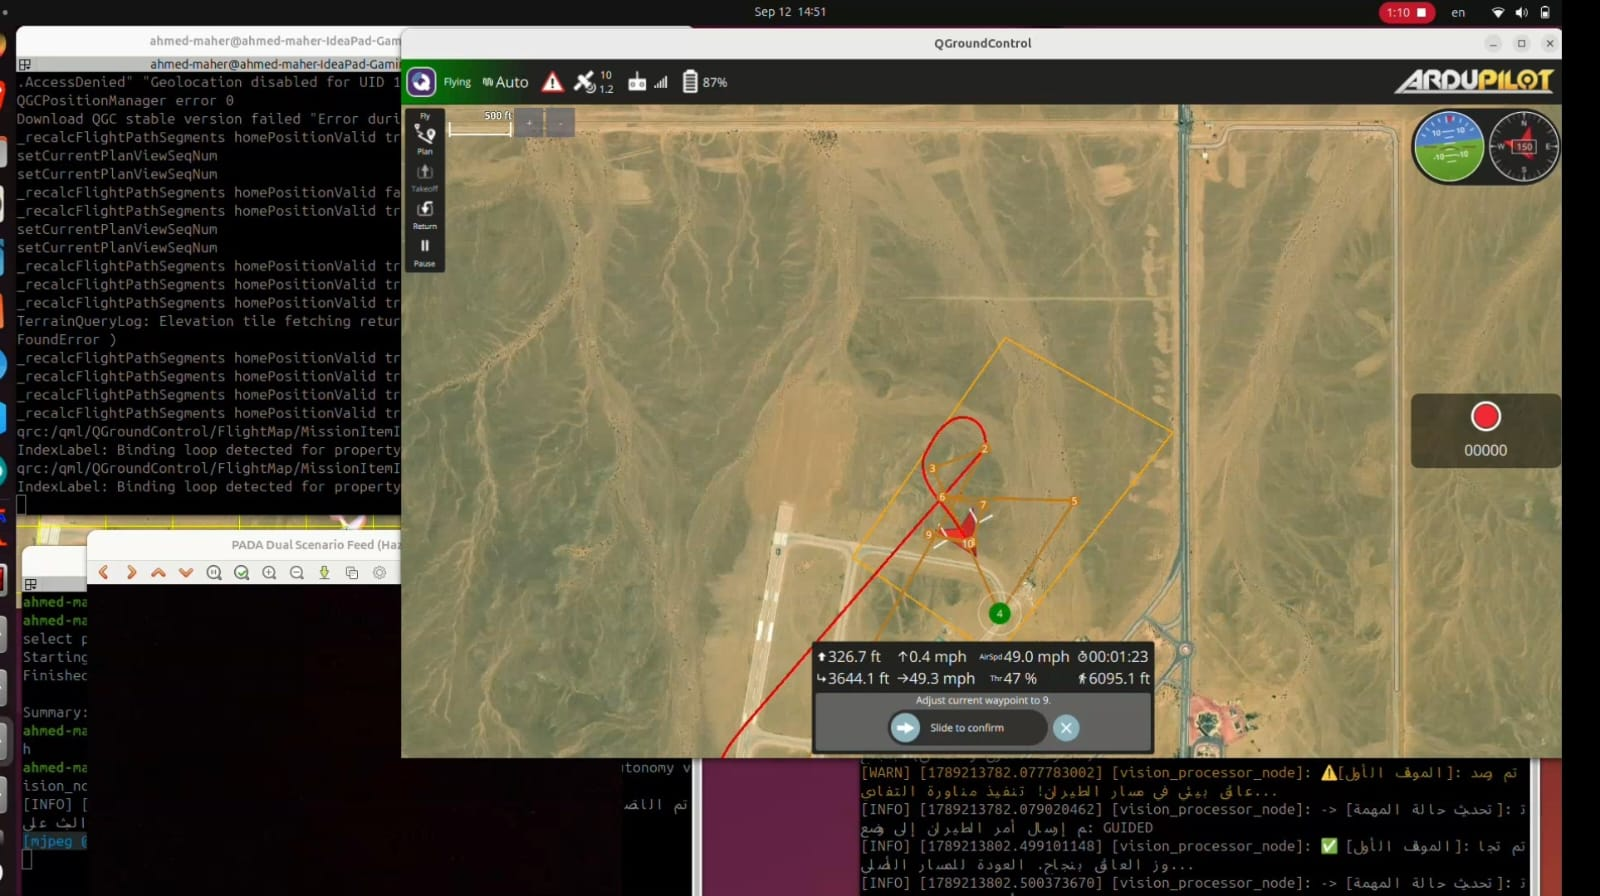
\includegraphics[width=\textwidth]{images/AUTO_MODE.jpeg}
        \caption{AUTO Mode execution.}
    \end{minipage}
    \hfill
    \begin{minipage}{0.32\textwidth}
        \centering
        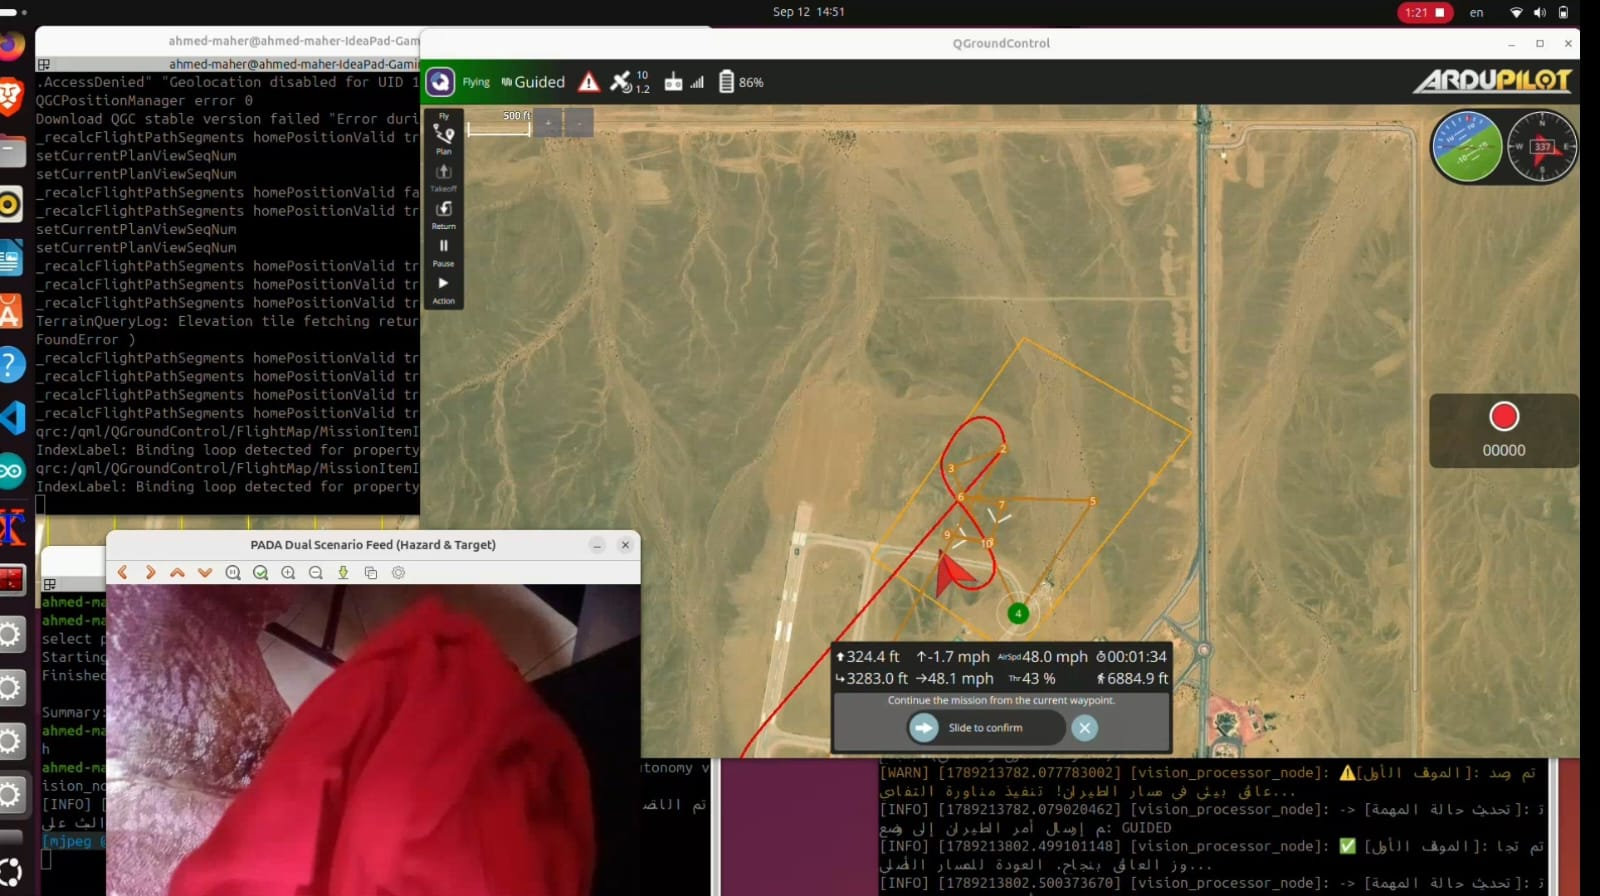
\includegraphics[width=\textwidth]{images/GUIDED_MODE.jpeg}
        \caption{GUIDED Mode hazard evasion.}
    \end{minipage}
    \hfill
    \begin{minipage}{0.32\textwidth}
        \centering
        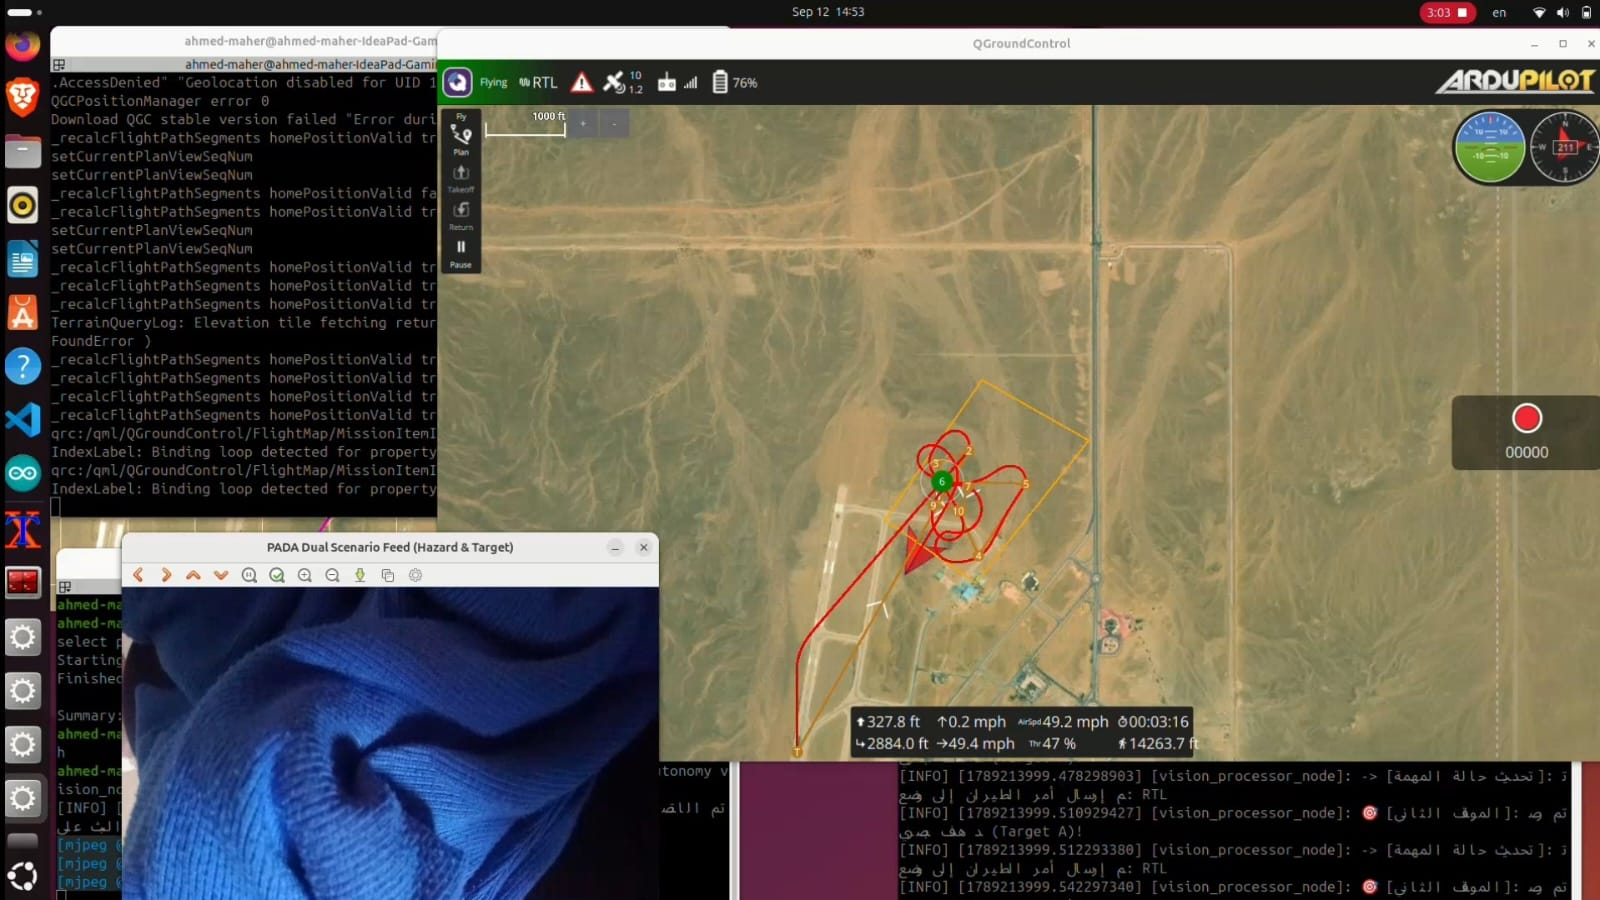
\includegraphics[width=\textwidth]{images/RTL_MODE.jpeg}
        \caption{RTL Mode command response.}
    \end{minipage}
\end{figure}

% ============================================================
% SECTION 6: MANUFACTURING PLAN
% ============================================================

\section{Manufacturing Plan}
The manufacturing strategy utilizes laser-cut balsa wood components:
\begin{itemize}
    \item \textbf{Material Sourcing:} Standard balsa planks ($\SI{1000}{\milli\meter} \times \SI{100}{\milli\meter} \times \SI{5}{\milli\meter}$).
    \item \textbf{Digital Preparation:} CAD models exported as 2D vector layouts.

    \begin{figure}[H]
        \centering
        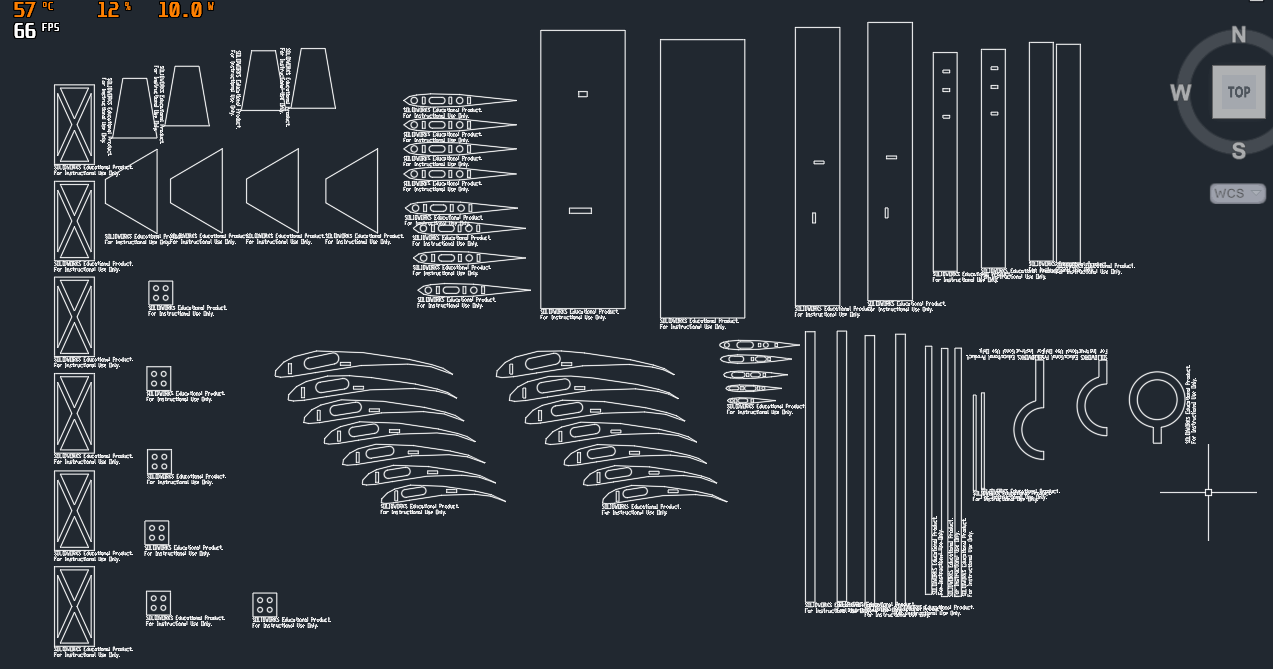
\includegraphics[width=0.55\textwidth]{images/All Components CAD.png}
        \caption{Full 2D manufacturing CAD cutting sheet.}
        \label{fig:manu_inst}
    \end{figure}

    \item \textbf{Laser Cutting:} Interlocking tabs and slots cut with high precision.
    \item \textbf{Assembly:} Structural alignment and gluing followed by avionics integration.
\end{itemize}

% ============================================================
% SECTION 7: BONUS / APPENDIX
% ============================================================

\section{Bonus: System Execution Logs}

\subsection{Software Execution Logs \& Terminal Outputs}
Software logs confirm stable, non-blocking operational loops across both active nodes during SITL flight tests:

\subsubsection{Camera Publisher Node Output}
\begin{lstlisting}[language=bash, caption={Terminal output from camera\_publisher\_node demonstrating initialization and active publishing.}]
[INFO] [1726240100.123456] [camera_publisher_node]: Initializing Camera Publisher Node...
[INFO] [1726240100.456789] [camera_publisher_node]: Connecting to camera stream at: http://192.168.1.50:8080/video
[INFO] [1726240101.012345] [camera_publisher_node]: Camera stream successfully opened (Buffer size set to 1).
[INFO] [1726240101.050000] [camera_publisher_node]: Publishing frames to '/camera/image_raw' at 30 FPS...
[INFO] [1726240130.050000] [camera_publisher_node]: Published 900 frames successfully. Stream stable.
\end{lstlisting}

\subsubsection{Vision Processor Node \& MAVROS Execution Logs}
\begin{lstlisting}[language=bash, caption={Terminal log capturing real-time color detection, area filtering, and flight mode service responses.}]
[INFO] [1726240102.100000] [vision_processor_node]: Subscribed to '/camera/image_raw'. Waiting for MAVROS service...
[INFO] [1726240102.350000] [vision_processor_node]: Connected to service '/mavros/set_mode'. System READY.
[INFO] [1726240105.000000] [vision_processor_node]: [STATE] Mission active. Aircraft operating in AUTO mode.

% --- Hazard Detection (Red Target) ---
[WARN] [1726240115.220000] [vision_processor_node]: [HAZARD DETECTED] Red contour area: 1850 px (Threshold: 600 px).
[INFO] [1726240115.225000] [vision_processor_node]: Requesting flight mode switch to 'GUIDED'...
[INFO] [1726240115.280000] [vision_processor_node]: Service call SUCCESS: Mode set to 'GUIDED' (MAVROS response: True).

% --- Hazard Resolution & Recovery ---
[INFO] [1726240125.100000] [vision_processor_node]: [CLEAR] Hazard removed from view. Area: 120 px (< 600 px).
[INFO] [1726240125.105000] [vision_processor_node]: Reverting flight mode to 'AUTO'...
[INFO] [1726240125.150000] [vision_processor_node]: Service call SUCCESS: Mode set to 'AUTO' (Resuming mission).

% --- Mission Command (Blue Target) ---
[INFO] [1726240140.050000] [vision_processor_node]: [TARGET A DETECTED] Blue contour area: 2410 px (Threshold: 600 px).
[INFO] [1726240140.055000] [vision_processor_node]: Requesting flight mode switch to 'RTL'...
[INFO] [1726240140.110000] [vision_processor_node]: Service call SUCCESS: Mode set to 'RTL' (MAVROS response: True).
\end{lstlisting}

\subsubsection{Log Analysis \& System Verification}
\begin{itemize}
    \item \textbf{Latency:} Sub-100ms elapsed time between visual hazard detection and MAVROS mode execution.
    \item \textbf{Noise Filtering:} Background reflections ($120\text{ px}$) were correctly filtered below the $600\text{ px}$ threshold without causing mode state chatter.
\end{itemize}

\end{document}